\definecolor{mygreen}{rgb}{0,0.6,0}
\definecolor{mygray}{rgb}{0.5,0.5,0.5}
\definecolor{mymauve}{rgb}{0.58,0,0.82}

%%%%%%%%%%%%%%%%%%%%%%%%%%%%%%%%%%%%%%%%%%%%%%%%%%%%%%%%%%%%%%%%%%%%%%%%%%%%%
% parámetros para configurar el formato del código en los entornos lstlisting
%%%%%%%%%%%%%%%%%%%%%%%%%%%%%%%%%%%%%%%%%%%%%%%%%%%%%%%%%%%%%%%%%%%%%%%%%%%%%
\lstset{ %
  backgroundcolor=\color{white},   % choose the background color; you must add \usepackage{color} or \usepackage{xcolor}
  basicstyle=\footnotesize,        % the size of the fonts that are used for the code
  breakatwhitespace=false,         % sets if automatic breaks should only happen at whitespace
  breaklines=true,                 % sets automatic line breaking
  captionpos=b,                    % sets the caption-position to bottom
  commentstyle=\color{mygreen},    % comment style
  deletekeywords={...},            % if you want to delete keywords from the given language
  escapeinside={(*@}{@*)},          % if you want to add LaTeX within your code
  %extendedchars=true,              % lets you use non-ASCII characters; for 8-bits encodings only, does not work with UTF-8
  %frame=single,	                % adds a frame around the code
  keepspaces=true,                 % keeps spaces in text, useful for keeping indentation of code (possibly needs columns=flexible)
  keywordstyle=\color{blue},       % keyword style
  language=[ANSI]C,                % the language of the code
  %otherkeywords={*,...},           % if you want to add more keywords to the set
  numbers=left,                    % where to put the line-numbers; possible values are (none, left, right)
  numbersep=5pt,                   % how far the line-numbers are from the code
  numberstyle=\tiny\color{mygray}, % the style that is used for the line-numbers
  rulecolor=\color{black},         % if not set, the frame-color may be changed on line-breaks within not-black text (e.g. comments (green here))
  showspaces=false,                % show spaces everywhere adding particular underscores; it overrides 'showstringspaces'
  showstringspaces=false,          % underline spaces within strings only
  showtabs=false,                  % show tabs within strings adding particular underscores
  stepnumber=1,                    % the step between two line-numbers. If it's 1, each line will be numbered
  stringstyle=\color{mymauve},     % string literal style
  tabsize=2,	                   % sets default tabsize to 2 spaces
  title=\lstname,                  % show the filename of files included with \lstinputlisting; also try caption instead of title
  morecomment=[s]{/*}{*/}
}

\chapter{Diseño e implementación} % Main chapter title
\label{Chapter3} % Change X to a consecutive number; for referencing this chapter elsewhere, use \ref{ChapterX}

En este capítulo se describen los aspectos más relevantes del diseño e implementación de la plataforma. Inicialmente se presenta su arquitectura en donde se describen sus componentes e interacciones. Luego se describe el proceso de despliegue de la infraestructura de soporte, tanto en el ambiente de desarrollo como en el de producción. Posteriormente se enfatiza en tarea de etiquetado de datos, incluyendo los problemas y soluciones enfrentados. Finalmente se presentan los desafíos más importantes interactuados con respecto al desarrollo de la aplicación web y el despliegue de la misma junto con los modelos de detección.

%----------------------------------------------------------------------------------------
%	SECTION 1
%----------------------------------------------------------------------------------------
\section{Arquitectura de la plataforma}
\label{sec:arquitectura}

El objetivo principal de este trabajo fue brindar un producto para el servicio de arbolado, en donde se les permita consultar el estado de la plaga en base a imágenes aéreas. Para ello, se diseñó y desarrolló la plataforma de la figura \ref{fig:plataforma}, la cual integra varios módulos con el fin de soportar todos los procesos relacionados con el desarrollo del software.

\begin{figure}[H]
  \centering
  \includegraphics[scale=0.1]{./Figures/diagrama_de_bloques_modulos_e_interacción.png}
  \caption{Diagrama de arquitectura del sistema de monitoreo.}
  \label{fig:plataforma}
\end{figure}

El enfoque se basó en un sistema modular, que favorece la encapsulación de funcionalidades específicas dentro de componentes con una única responsabilidad (SRP, sigla del inglés \textit{Single Responsibility Principle} \citep{soni_software_2024}). Esto facilita la mantenibilidad y escalabilidad del sistema, permitiendo que cada módulo pueda ser desarrollado, probado, intercambiado y desplegado de manera independiente. Cada módulo desempeña un papel específico en varios de los procesos transversales de la ingeniería de software, como lo es la gestión de datos, la seguridad, el respaldo de información y el despliegue de aplicaciones.

La estructura modular de la plataforma permite que se puedan agregar otros módulos en el futuro, como por ejemplo, un módulo de información georreferenciada, que centralice las referencias de las palmeras y permita visualizaciones internamente utilizando herramientas como QGIS \citep{wikipedia_qgis_2025} o un módulo reportes, que gestione todos los resultados de los entrenamiento de los modelos, con herramientas como MlFlow \citep{zaharia_accelerating_2018}. Esto posibilita que la plataforma pueda evolucionar y adaptarse a nuevas necesidades y tecnologías, asegurando su relevancia a largo plazo.

Uno de los principales objetivos al definir la arquitectura, fue que los módulos representen responsabilidades que ya están resueltas por software existente en la infraestructura de la IM. Esto permite que, en un futuro, estos módulos puedan ser reemplazados por el software ya utilizado en la IM, o incorporados como servicios adicionales aquellos que no existen, como el módulo de IA.

La comunicación se basa en protocolos ligeros como REST \citep{wikipedia_protocolo_2024}, que generan un bajo acoplamiento y una alta cohesión entre módulos, aunque también se utilizan otros protocolos como LDAP para la gestión de usuarios y permisos, asi como OIDC para la autenticación y autorización de la aplicación web (Mis palmeras).

El módulo de seguridad permite la administración de usuarios y permisos. Esto garantiza que solo los usuarios autorizados tengan acceso a la información sensible. Este módulo se basa en el protocolo LDAP, que favorece una gestión centralizada de autenticación y autorización. Adicionalmente, el módulo puede ser sustituido por el software utilizado en la IM (WSO2 \citep{wso2_deliver_nodate}) o directamente interactuar con este (WSO2 puede comunicarse mediante el protocolo LDAP).

El módulo de respaldo de datos cerciora que los datos estén siempre disponibles y que se puedan recuperar en caso de pérdida. En este caso es extremadamente importante este módulo, dado que el costo de obtener los datos etiquetados es muy alto, por lo que es información muy valiosa y esto aumenta el riesgo. El objetivo principal de este módulo pasa por gestionar procesos de respaldo y recuperación de datos. Al ser un módulo independiente, puede ser sustituido por otro software de respaldo, como por ejemplo: Restic \citep{restic_restic_nodate} o Bacula \citep{bacula_documentation_nodate}.

El módulo gestor de datos es el encargado de almacenar los metadatos de las imágenes. Está conformado por una base de datos orientada a documentos, que permite almacenar varios tipos de datos (explicado en la sección \ref{sec:gestionRepoDatos}). Esta forma de almacenamiento, que mejora la eficiencia, facilita la gestión de grandes volúmenes de información. Asimismo, esta estructura también soluciona el desafío guardar las etiquetas generadas por los usuarios en el proceso de etiquetado de datos.

El módulo de etiquetado de datos permite ejecutar el proceso de etiquetado de imágenes y se comunica tanto con el módulo de seguridad para el manejo de diferentes niveles de información. Su acoplamiento es muy bajo, con el objetivo de que pueda ser sustituido por otro software de etiquetado, dado la gran variedad de herramientas disponibles en el mercado. Se comunica con el módulo de repositorio de objetos para obtener las imágenes a etiquetar y con el módulo de seguridad para gestionar los usuarios y permisos. Asimismo, este módulo también brinda una interfaz gráfica para que el usuario pueda realizar el etiquetado de manera sencilla.

El módulo de calidad de datos se ocupa de realizar un análisis cualitativo de los datos, lo que mejora la eficiencia de los modelos al utilizar datos de alta calidad. Este módulo permite que un equipo de control de calidad pueda analizar y generar informes específicos sobre los datos, lo que habilita una traza y evolución de lás imágenes, esencial en proyectos de VPC donde la variable temporal afecta el resultado de las predicciones, como lo es este trabajo. Este módulo también se comunica con el usuario mediante una interfaz gráfica que permite una correcta gestión de la calidad de los datos.

El módulo de repositorio de objetos es el responsable del almacenamiento y gestión de las imágenes, en este caso las generadas por drones. Este módulo administra grandes volúmenes de datos y garantiza la disponibilidad continua de esta información mediante APIs. Para esta tarea, usualmente se utilizan sistemas de almacenamiento de objetos como Amazon S3 \citep{amazon_web_services_aws_nodate} o algún otro proveedor de nube. La comunicación con otros módulos se realiza mediante APIs REST, lo que permite una integración sencilla y eficiente.

El módulo de "Mis palmeras" contiene la aplicación web principal del sistema. Es la cara visible del sistema y permite a los usuarios interactuar con la información de manera sencilla. Esta aplicación tiene el objetivo de mostrar el estado de la plaga en base a las imágenes aéreas y los resultados de los modelos de detección. Se comunica con el módulo de seguridad para la autenticación y autorización de los usuarios, utiliza componentes del módulo de utilidades (como las transformaciones entre varios formatos) y solicita predicciones al módulo de IA mediante una API REST. Está orientado a mostrar información georreferenciada y actualmente su acoplamiento con el módulo IA es fuerte, sin embargo, en un futuro se podría mejorar esta interacción mediante una API REST, lo que permitiría una mayor flexibilidad y escalabilidad del sistema.

El módulo utilidades centraliza aplicaciones utilizadas en varias tareas, como la actualización, migración y generación de datos que usualmente son insumos para los procesos de entrenamiento. Este módulo realiza tareas específicas que no están directamente relacionadas con el proceso de detección, pero que son necesarias para el correcto funcionamiento del sistema. Un ejemplo de esto es la aplicación que efectúa \textit{web scrapping} del sistema de información geográfica de la IM, para descargar las imágenes de los vuelos allí publicadas y guardarlas en el repositorio de imágenes.

Finalmente, el módulo de IA se encarga de cumplir con los procesos asociados al entrenamiento y despliegue de los modelos. Tiene el objetivo de manejar sus el ciclos de vida, desde su desarrollo hasta su despliegue en producción. Incluye la ejecución de experimentos. Actualmente no expone una API para solicitar predicciones, lo que lo hace menos flexible (hay que estar gestionando los artefactos de un módulo a otro).

Un resumen de las interfaces de comunicación con el exterior de la plataforma se puede observer en la figura \ref{fig:interfaces-externas}, en donde se puede observar que existen cuatro interfaces de comunicación externa, tres interfaces webs y una API REST para realizar el \textit{web scrapping}.

\begin{figure}[H]
  \centering
  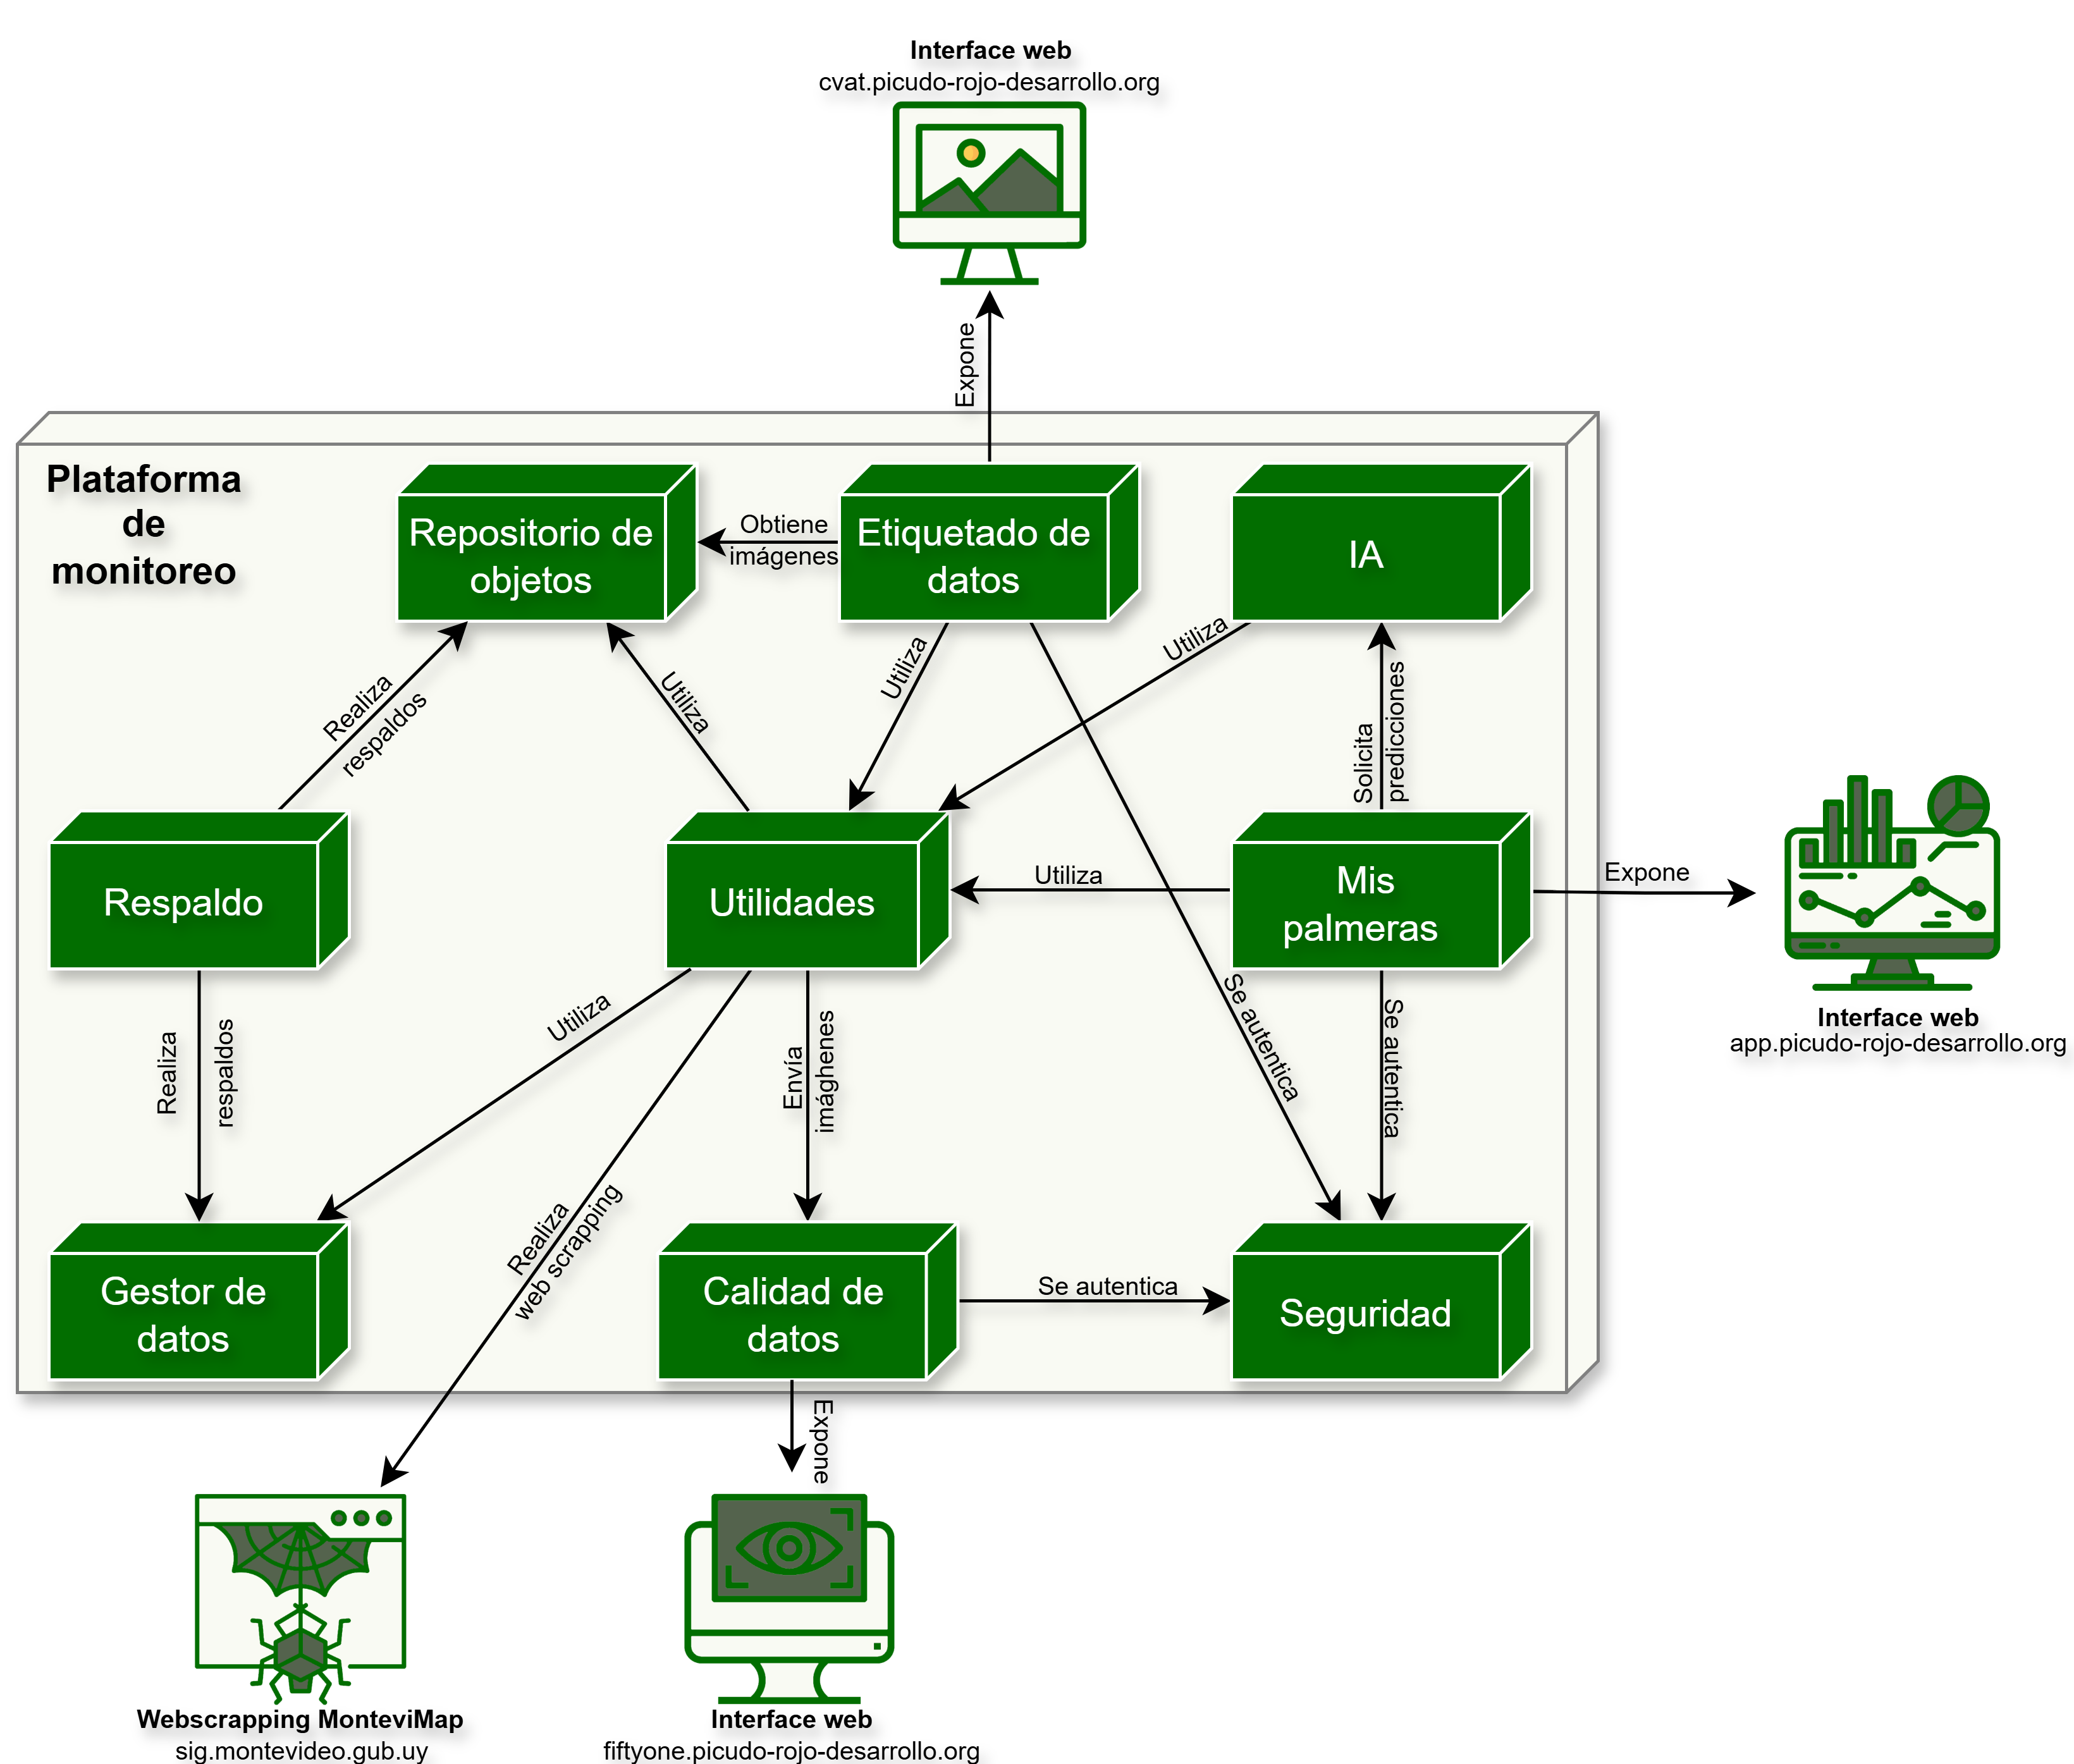
\includegraphics[scale=0.115]{./Figures/diagrama_de_bloques_interfaces_externas.png}
  \caption{Diagrama de interfaces externas.}
  \label{fig:interfaces-externas}
\end{figure}

Si bien el objetivo del trabajo es la detección del picudo rojo, fue necesario el desarrollo de esta plataforma de soporte, principalmente para el etiquetado de datos, dado que se necesitaba disponibilizar las imágenes a los usuarios encargados de esta tarea, para recién luego poder entrenar los modelos de detección.

%	SECTION 2
%----------------------------------------------------------------------------------------

\section{Despliegue de la infraestructura de soporte}
\label{sec:despliegue_infraestructura}

% Hablar de la comparación entre CVAT y Label Studio?
% Hablar de la dificultad de desplegar CVAT?
% Hablar de virtualbox, de su problema de compatibilidad con mongodb?

El objetivo principal fue encontrar soluciones de código abierto para cada módulo, y si una solución era compatible con la infraestructura de la IM, se priorizó su uso.

Los ambientes de trabajo se dividieron en dos dominios: desarrollo y producción. El primero se utilizó para el desarrollo y pruebas preliminares, mientras que el segundo, se destinó al despliegue final del sistema. Se utilizó una configuración de espejo, en donde ambos ambientes tenían la misma estructura y componentes, lo que facilitó la transición entre ellos. La principal diferencia entre ambos ambientes radica en la configuración de seguridad y rendimiento, adaptada a las necesidades específicas de cada entorno. Las herramientas seleccionadas se pueden observar en la figura \ref{fig:infra-desarrollo}.

\begin{figure}[H]
  \centering
  \includegraphics[scale=0.12]{./Figures/diagramas_de_bloques_tecnologías.png}
  \caption{Diagrama de la plataforma de monitoreo.}
  \label{fig:infra-desarrollo}
\end{figure}

Una descripción de las tecnologías utilizadas en cada módulo se puede observar en la tabla \ref{tab:tecnologias}.

\begin{table}[H]
  \centering
  \caption[Tecnologías utilizadas]{Tecnologías utilizadas por módulo \footnotemark.}
  % \begin{adjustbox}{width=\textwidth}
  \begin{tabular}{l l l}
    % \begin{tabular}{{l p{4cm} p{4cm}}}
    \toprule
    \textbf{Módulo}  & \textbf{Herramienta}        & \textbf{Tecnología/Descripción}    \\ \hline
    \midrule
    Seguridad        & LLDAP                       & LDAP                               \\ \hline
    Seguridad        & \makecell[l]{LDAP                                                \\Self Serivce Password \citep{ltb_project_ldap_nodate}} & PHP                             \\ \hline
    Seguridad        & \makecell[l]{KeepAlive                                           \\(Scripts personalizados)}      & Bash                            \\ \hline
    Seguridad        & Keycloak                    & OIDC, OAuth2                       \\ \hline
    Respaldo         & \makecell[l]{Backup-Restore                                      \\(Scripts personalizados)} & Bash                            \\ \hline
    Gestor de datos  & MongoDB                     & Base de datos NoSQL                \\ \hline
    \makecell[l]{Etiquetado                                                             \\de datos}          & CVAT                                    & \makecell[l]{React, Django,                      \\PostgreSQL}                     \\ \hline
    Calidad de datos & FiftyOne                    & \makecell[l]{React, Python (ASGI), \\MongoDb}                        \\ \hline
    \makecell[l]{Repositorio                                                            \\de objetos}       & MinIO                                   & \makecell[l]{Almacenamiento \\de objetos }      \\ \hline
    Mis palmeras     & Angular, FastAPI            & Aplicación web                     \\ \hline
    Utilidades       & \makecell[l]{Web scrapping,                                      \\anotaciones}  & \makecell[l]{Python, BeautifulSoup, \\CVAT SDK}    \\ \hline
    IA               & \makecell[l]{YoloV11,                                            \\anotadores}                     & \makecell[l]{Python, PyTorch, \\Ultralytics}    \\ \hline
    \makecell[l]{Orquestación                                                           \\de contenedores} & Docker Compose                          & Docker                          \\ \hline
    \makecell[l]{Infraestructura                                                        \\como código}  & Vagrant                                 & VirtualBox \citep{wikipedia_virtualbox_2025}                     \\ \hline
    Proxy reverso    & Traefik                     & Traefik                            \\ \hline
    \bottomrule
    \hline
  \end{tabular}
  % \end{adjustbox}
  \label{tab:tecnologias}
\end{table}

El despliegue de la infraestructura de producción pasó por tres etapas de adaptación:

\begin{itemize}
  \item Despliegue inicial en la nube pública: se utilizó la nube pública de Scaleway para el despliegue inicial, aprovechando su capa gratuita para almacenamiento de objetos (\textit{object storage}), la cual permite almacenar hasta 80 GB de datos. Esto permitió validar la arquitectura y las interacciones entre los módulos en un entorno realista. Surgieron varios desafíos, como la correcta selección de las instancias de cómputo adecuadas para CVAT, la configuración de la red para permitir el acceso externo y la gestión de costos asociados al uso de recursos en la nube. Además, para el despliegue de CVAT se gestionó certificados SSL utilizando Let's Encrypt \citep{aas_lets_2019}, lo que agregó otra capa de complejidad al proceso de configuración inicial. Sin embargo, a medida que el proyecto avanzaba, los costos aumentaron significativamente, por lo que se decidió migrar a una infraestructura semigestionada.
  \item Despliegue semigestionado: se optó por una infraestructura semigestionada, utilizando un servidor físico local. Esto permitió reducir costos y tener un mayor control sobre los recursos. Se utilizó Ngrok \citep{ngrok_inc_ngrok_nodate} (un servicio de \textit{tunneling}) para exponer los servicios a internet de manera segura, lo que facilitó el acceso remoto a la plataforma. Esta etapa implicó desafíos relacionados con la configuración de la red interna, la gestión de certificados SSL y la optimización del rendimiento de los servicios desplegados. Si bien se disminuyeron los costos en comparación con la nube pública, no se llegó a un costo aceptable, dado que Ngrok tiene un trafico de salida limitado y como se trabajó con imágenes de alta resolución, este límite se alcanzaba rápidamente. Por lo tanto, se decidió migrar a una infraestructura auto-gestionada como solución final.
  \item Despliegue final (autogestionado): existieron muchos desafíos en esta etapa, desde la configuración de servicios \textit{no-ip} para gestionar un DNS dinámico, hasta la correcta configuración de los certificados SSL. Para esto, se contrató un dominio en Cloudflare  \citep{cloudflare_conecta_nodate} (picudo-rojo.org), se configuró Traefik \citep{traefik_labs_traefik_nodate} como proxy reverso y se realizaron diversas configuraciones para exponer de forma segura una máquina virtual por medio de Vagrant. Esta etapa finalizó con el despliegue exitoso de la plataforma en un entorno autogestionado, asegurando su disponibilidad y rendimiento óptimo.
\end{itemize}

El ambiente de desarrollo se puede reproducir en cualquier máquina que tenga instalado Vagrant y VirtualBox. La máquina anfitriona puede ser cualquier sistema operativo, ya sea Windows, macOS o Linux. Esto permite que cualquier desarrollador pueda tener el mismo ambiente de desarrollo en su máquina local, lo que facilita la colaboración y el trabajo en equipo, simplemente clonando el repositorio \citep{bruno_masoller_brunomaso1uba-ceia_nodate} mediante Git y luego importar el proyecto utilizando un IDE \citep{wikipedia_entorno_2025}. En este caso, se utilizó Visual Studio Code.

Una vez importado el proyecto, la estructura de directorios emula cada módulo del proyecto de la siguiente manera:

\begin{lstlisting}[label=cod:vControl,caption=Estructura de directorios utilizada., literate={├}{{\textSFviii}}1 {─}{{\textSFx}}1 {└}{{\textSFii}}1 {│}{{\textSFxi}}1]  % Start your code-block

desarrollo/
├── modulo-aplicaciones-web/
│   ├── entrypoint/ 
│   ├── mis-palmeras/
│   └── landing-page/
├── modulo-calidad-datos/
│   └── fiftyone/
├── modulo-etiquetado-datos/
│   └── cvat/
├── modulo-gestor-datos/
│   └── mongo/
├── modulo-ia/
│   ├── modulo_ia/
│   └── ...
├── modulo-utilidades/
│   ├── modulo_utils/
│   └── ...
├── modulo-repositorio-objetos/
│   └── minio/
├── modulo-respaldo/
│   └── scripts/
├── modulo-seguridad/
│   ├── keepalive/
│   ├── keycloak/
│   ├── ssp/
│   └── lldap/
├── vagrant-scripts/
├── readme.md
└── Vagrantfile

\end{lstlisting}

Los módulos IA y utilidades, se estructuran utilizando \textit{Cookiecutter Data Science} \citep{drivendata_cookiecutter_nodate}, que es una plantilla para proyectos de ciencia de datos. Esta estructura facilita la organización del código, datos y documentación, promoviendo buenas prácticas en el desarrollo de proyectos de ciencia de datos. Estos módulos también cuentan con Poetry \citep{eustace_poetry_nodate} como gestor de dependencias y entornos virtuales, lo que permite aislar las dependencias de cada proyecto y evitar conflictos entre ellas. Finalmente, también posibilita empaquetar y distribuir las funcionalidades desarrolladas como librerías reutilizables.

En ingeniería de software es importante asegurar la reproducibilidad de los ambientes de trabajo. Una de las herramientas utilizadas con este objetivo fue Docker, el cual habilita crear contenedores que encapsulan una aplicación y sus dependencias. Esto asegura un entorno de ejecución uniforme y reproducible en diferentes sistemas. Para la orquestación de múltiples contenedores se utilizó Docker Compose, que brinda una infraestructura en entornos complejos en donde interactúan varias aplicaciones.

Cada directorio tiene su propio archivo de Docker Compose (\lstinline[language=sh]|docker-compose.yml|) que habilita el despliegue de las herramientas del módulo. Esto, además de las ventajas mencionadas anteriormente en la sección \ref{sec:arquitectura}, también permite que cada componente pueda ser desarrollado y probado de manera independiente (con sus debidos \textit{stubs} \citep{wikipedia_talon_2025} o \textit{mocks} \citep{wikipedia_objeto_2024}), lo que reduce el \textit{Lead Time} \citep{wikipedia_lead_2025}. Estos archivos de configuración pueden ser adaptados a distintas situaciones. Por ejemplo, el archivo \lstinline[language=sh]|docker-compose.yml| de MinIO fue adaptado para que, si no existe el \textit{bucket} llamado "picudo-rojo-bucket", se cree automáticamente.

Asimismo, cada módulo tiene sus variables de entorno definidos como archivos \lstinline[language=sh]|.env| su directorio raíz. Esto permite separar la configuración de los distintos ambientes para cada módulo. En este sentido, concede la fácil transición entre el ambiente de desarrollo y el ambiente de producción.

Aunque Docker permite crear contenedores que emulan el ambiente de producción, esto no es suficiente para asegurar la reproducibilidad de este dominio en el entorno de desarrollo. Esto se debe a que Docker se ejecuta sobre una plataforma, que puede ser diferente en cada máquina. Por lo tanto, es necesario utilizar una herramienta que permita crear y gestionar la infraestructura de soporte de manera uniforme y reproducible. Para esto se utilizó Vagrant.

Vagrant concede la habilidad de crear una o varias máquinas virtuales (VM, del inglés \textit{virtual machine}) que emulan una plataforma objetivo, en este caso, el ambiente de producción (Ubuntu 24). Se maneja con un archivo de configuración llamado Vagrantfile que brinda la posibilidad de realizar la definición de la configuración de la máquina virtual como \textit{infrastructure as a code}. Esto implica definir parámetros como la cantidad de memoria, el sistema operativo o las aplicaciones a instalar. Se puede utilizar una imagen de un sistema operativo ya configurado o crear una desde cero. En este caso se utilizó una imagen de Ubuntu 24.04 LTS \citep{progress_chefs_bento_bentoubuntu-2404_nodate}, del repositorio oficial de Vagrant \citep{hashicorp_hashicorp_nodate}, que incluye la mayoría de las herramientas necesarias para el desarrollo y despliegue del sistema. Esta imagen se puede utilizar en cualquier máquina que tenga instalado Vagrant y VirtualBox \citep{wikipedia_virtualbox_2025} (también se puede utilizar otro software de virtualización, como lo es Hyper-V \citep{meaghanlewis_informacion_2025} o VMWare \citep{wikipedia_vmware_2025}).

Asimismo, Vagrant también permite aprovisionar \textit{scripts} de configuración a las máquinas virtuales. Estos pueden ejecutarse al iniciar estas máquinas, lo que permite instalar y configurar las aplicaciones necesarias para poner el funcionamiento el sistema. En este caso, se utilizaron cuatro scripts de aprovisionamiento:

\begin{lstlisting}[label=cod:dd,caption=Scripts de vagrant utilizados., literate={├}{{\textSFviii}}1 {─}{{\textSFx}}1 {└}{{\textSFii}}1 {│}{{\textSFxi}}1]  % Start your code-block

vagrant-scripts/
├── 01-setup-network.sh
├── 02-install-dependencies.sh
├── 03-configure-firewall.sh
└── 04-start-dev-services.sh

\end{lstlisting}

En donde el último se encarga de iniciar los servicios dentro de cada módulo (usualmente se ejecuta mediante un script de shell el comando \lstinline[language=sh]|docker compose up|).

Una vez que se ejecuta el comando \lstinline[language=sh]|vagrant up|, se crea una máquina virtual (si ya no fue creada), se ejecutan los scripts de aprovisionamiento, lo que resulta en el ambiente de desarrollo listo para utilizarse. La ejecución del ambiente de producción es exactamente igual, pero con distintas configuraciones de archivos. Finalmente, se configuró el router para redirigir el tráfico de los puertos 80 y 443 de la máquina virtual, lo que permite acceder a la plataforma desde internet.

Entre los servicios que se inician se encuentran:

\begin{itemize}
  \item MongoDB: implementa la base de datos que permite almacenar metadatos de las imágenes ortorectificadas.
  \item MinIO: almacena las imágenes generadas por los drones.
  \item CVAT: se utiliza para etiquetar las imágenes almacenadas en el repositorio de objetos.
  \item FiftyOne: herramienta de análisis, organización, visualización y generación de informes sobre los datos.
  \item LLDAP: herramienta de gestión de usuarios y permisos, utilizada para administrar la seguridad del sistema.
  \item LDAP \textit{Self Service Password}: autoservicio de contraseñas (permite que los usuarios gestionen sus credenciales)
  \item \textit{Landing Page}: conjunto de herramientas basadas en tecnologías de desarrollo web (HTML, CSS, Javascript) que brindan información sobre el proyecto. Es la cara visible del sistema desde internet.
  \item Mis palmeras: aplicación web principal del sistema, que permite a los usuarios interactuar con la información de manera sencilla.
  \item Keycloak: sistema de gestión de identidad y acceso, que permite la autenticación y autorización de los usuarios.
  \item \textit{Entrypoint}: proxy reverso que expone el ambiente de desarrollo a internet o intranet para su fácil acceso.
\end{itemize}

Una vez iniciados los servicios, se puede acceder a la plataforma desde internet mediante el dominio \url{https://picudo-rojo.org}, lo que muestra la página de inicio (landing page) del sistema, como se observa en la figura \ref{fig:landing-page}.

% TODO: Crear la figura de la landing page
\begin{figure}[H]
  \centering
  
\includegraphics[scale=0.2]{./Figures/place-holder.png}
  \caption{Captura de pantalla de la página de inicio (landing page) del sistema.}
  \label{fig:landing-page}
\end{figure}

Desde allí, se puede acceder a la aplicación web principal (Mis palmeras) mediante el dominio \url{https://app.picudo-rojo.org}, al sistema de etiquetado de imágenes mediante el dominio \url{https://cvat.picudo-rojo.org} y la gestión de las contraseñas mediante el dominio \url{https://password.picudo-rojo.org}.

%----------------------------------------------------------------------------------------
%	SECTION 3
%----------------------------------------------------------------------------------------

\section{Obtención y gestión de las imágenes}
\label{sec:obtención-datos}

Posteriormente al despliegue de la infraestructura, se procedió a la obtención y gestión de las imágenes ortorectificadas. Para ello, se desarrolló un proceso de \textit{web scrapping} que automatiza la descarga de las imágenes desde el sistema de información geográfica (SIG) de la IM.

El SIG de la IM es un visor web de mapas que está construido con un framework que utiliza \textit{MapServer} \citep{mckenna_mapserver_2025}, en donde se permite navegar por capas de información geográfica. En la figura \ref{fig:sig-im} se puede observar una captura de pantalla, con la grilla de las imágenes de drones ortorectificadas.

\begin{figure}[H]
  \centering
  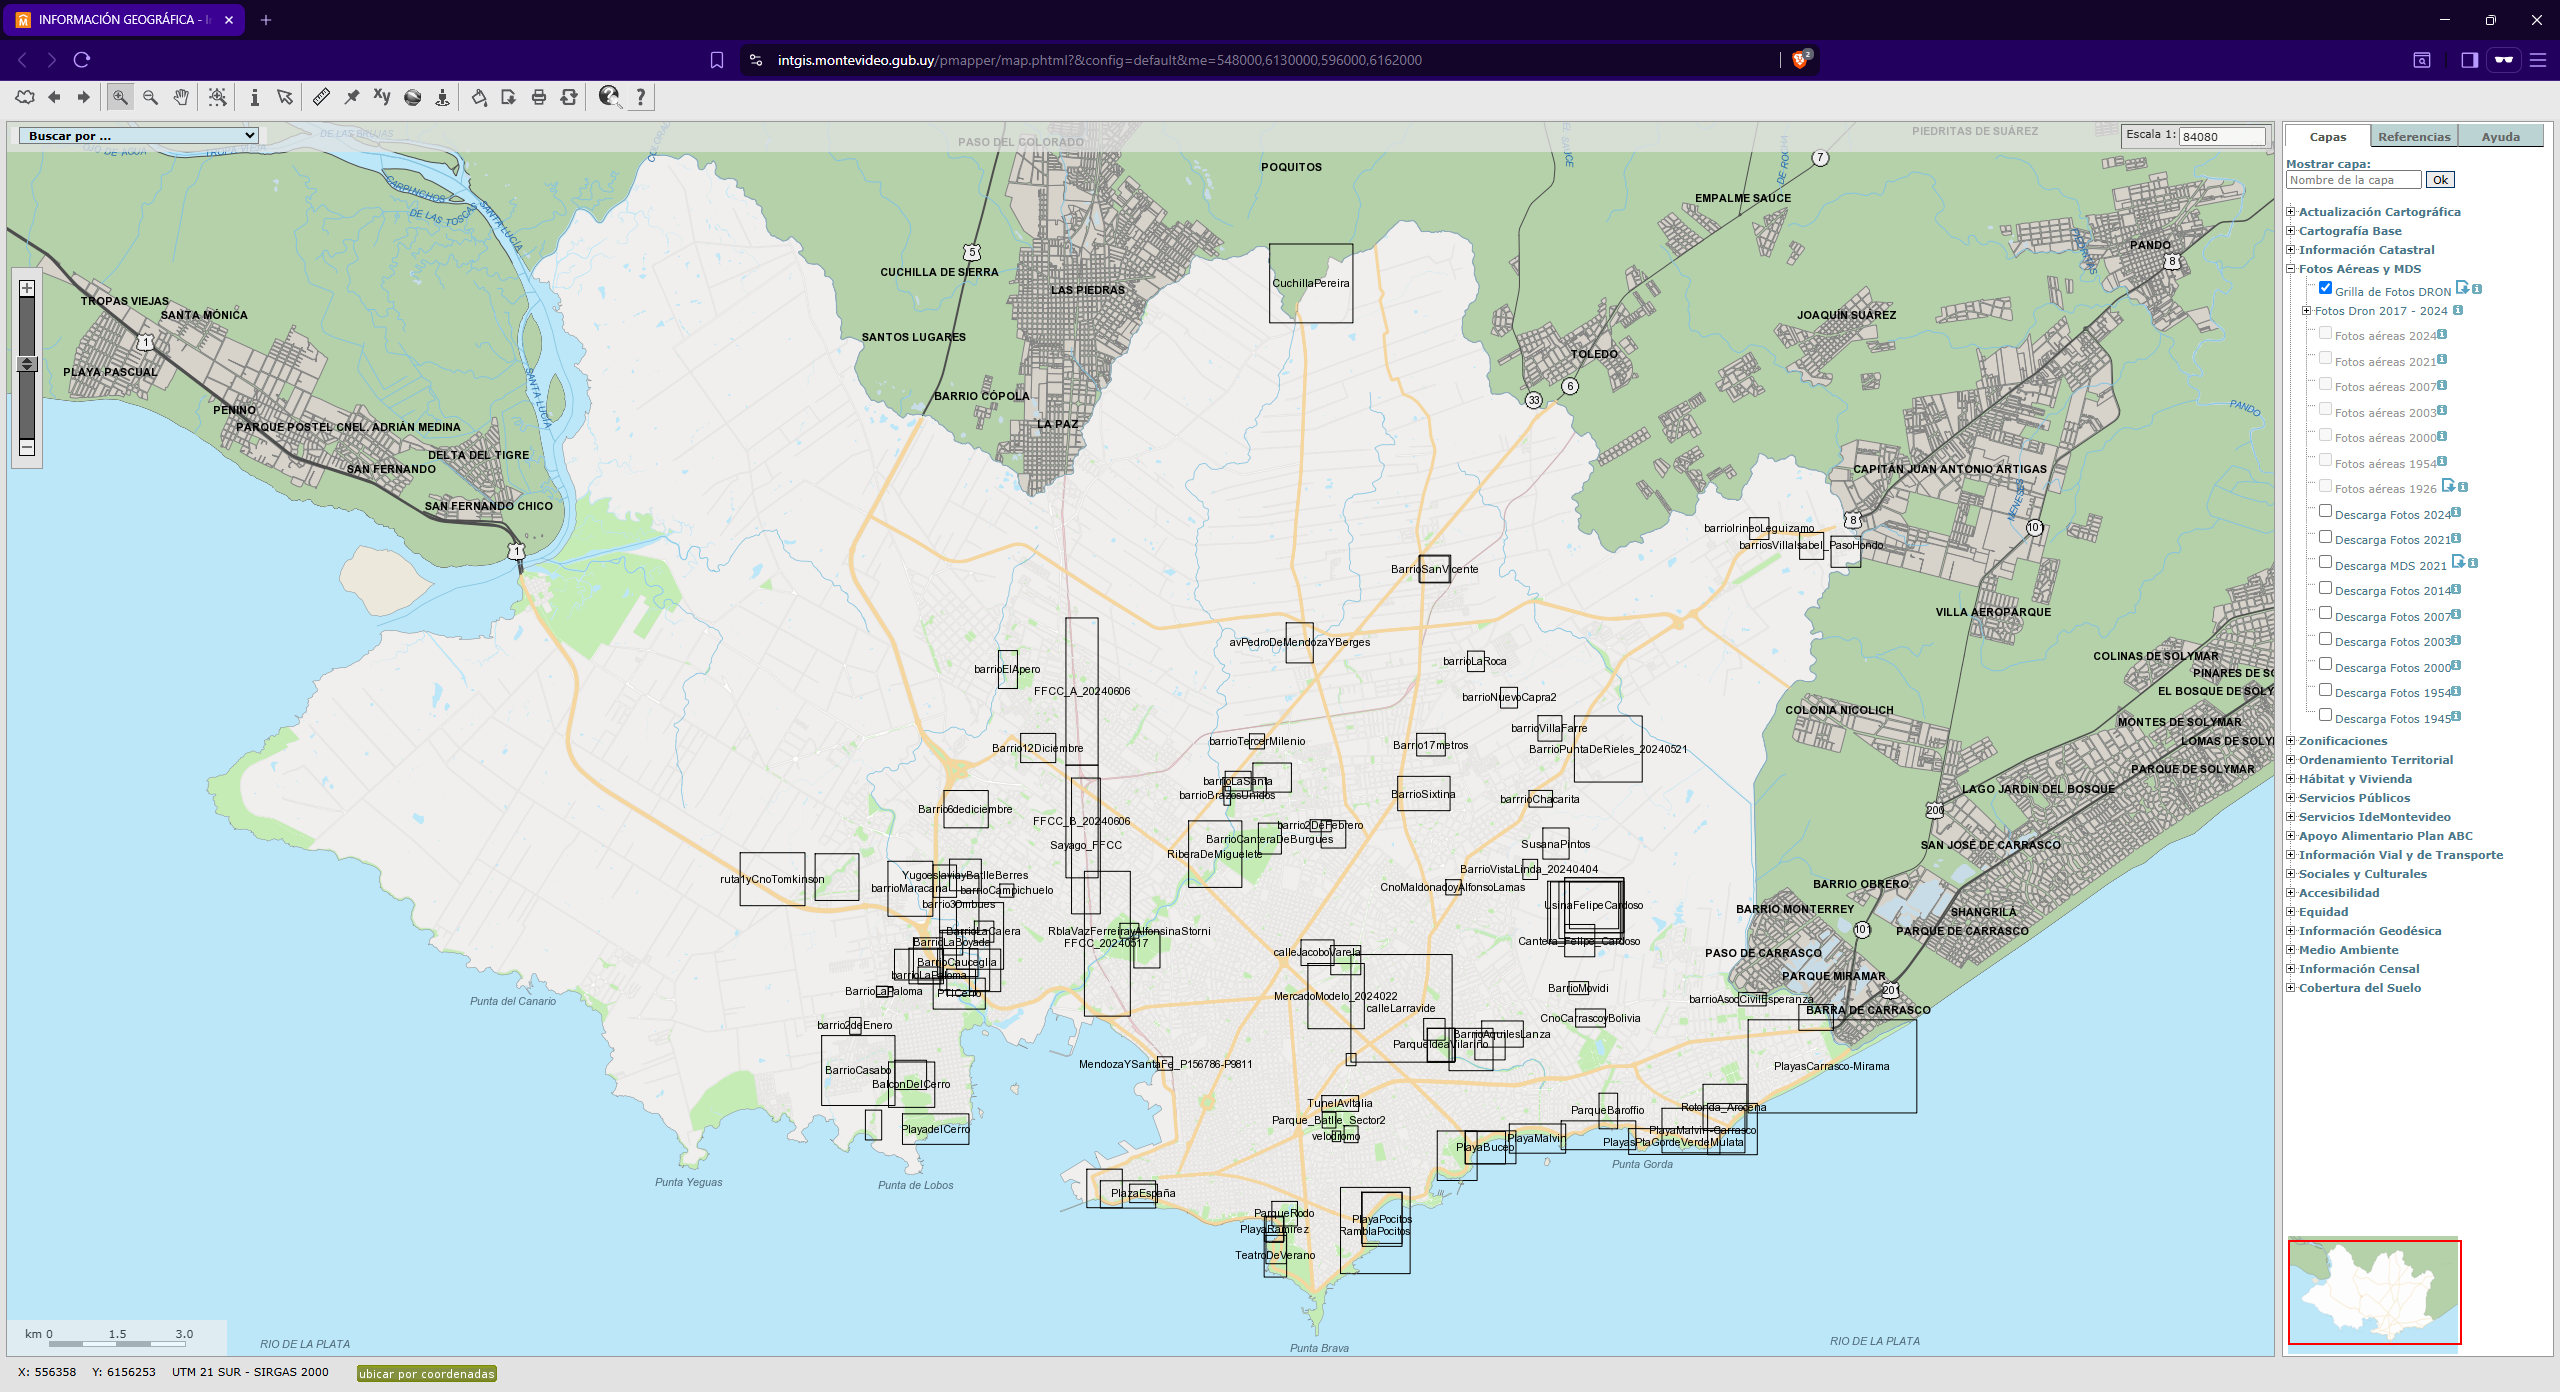
\includegraphics[scale=0.2]{./Figures/portada-sig.png}
  \caption{Captura de pantalla del SIG de la IM.}
  \label{fig:sig-im}
\end{figure}

Los vuelos fueron realizados con los drones DJI Phantom 4 RTK y DJI Mavic 2 Pro, ambos equipados con cámaras de alta resolución. Las imágenes capturadas por los drones fueron procesadas utilizando software especializado de fotogrametría, que incluye algoritmos avanzados para la corrección geométrica y la ortorectificación. Este proceso asegura que las imágenes sean precisas y estén alineadas correctamente con las coordenadas geográficas, lo que es esencial para su uso en análisis geoespaciales y aplicaciones de monitoreo ambiental.

Las imágenes ortorectificadas tienen una resolución espacial que varía entre 3 y 5 cm por píxel, dependiendo de la altitud del vuelo y las condiciones de captura; y están publicadas en formato vectorial (\lstinline[language=sh]|.jpg|) En la obtención de las imágenes, se incluyeron ambas resoluciones. 

El proceso de \textit{web scrapping} se desarrolló utilizando Python y la librería BeautifulSoup \citep{richardson_beautiful_2007}, que permite extraer información de páginas web de manera sencilla. El script automatiza la navegación por el SIG, identifica las imágenes ortorectificadas disponibles de los drones y las descarga en el repositorio de objetos (MinIO). Este proceso se ejecuta a demanda, lo que permite mantener el repositorio actualizado con las últimas imágenes disponibles en el SIG. Un desafío importante consistió en identificar la estructura HTML del SIG y extraer correctamente las URLs de las imágenes, lo que requirió un análisis detallado del código fuente de la página web, llegando a la conclusión de que las imágenes estaban almacenadas en un servidor externo, las cuales primero se generaban temporalmente y luego se permitía la descarga. Otro punto a destacar es que esta información estaba en un archivo Javascript que se generaba dinámicamente, lo que complicó la extracción de las URLs. Sin embargo, una vez superados estos desafíos, el proceso de \textit{web scrapping} se implementó con éxito, permitiendo la obtención eficiente de las imágenes ortorectificadas.

Un tema de importancia sobre las imágenes fue que el tamaño de las mismas era muy grande, lo que impidió que se cargaran tal cual en CVAT, dado que la herramienta tiene un límite de 65.000 píxeles en el lado más largo de la imagen. Por lo tanto, se decidió recortar las imágenes en fragmentos más pequeños, de \SI{4000}{}\,\texttimes\,\SI{4000}{\pixel}, lo que permitió que se pudieran cargar en CVAT sin problemas. Este proceso de recorte se automatizó para la descarga de todas las imágenes y se organizó el repositorio de objetos de manera estructurada, utilizando un esquema de nombres que facilita la identificación y gestión de las imágenes. Un ejemplo de los recortes realizados se puede observar en la figura \ref{fig:recortes-imagenes}.

\begin{figure}[H]
  \centering
  \includegraphics[scale=0.08]{./Figures/parches-ortomosaicos.png}
  \caption{Ejemplos de recortes de las imágenes ortorectificadas utilizadas.}
  \label{fig:recortes-imagenes}
\end{figure}

La organización de las imágenes en MinIO se realizó utilizando una nomenclatura altamente acoplada a CVAT, en donde cada carpeta representa un \textit{task} de CVAT. Esto permite que se puedan agregar \textit{tasks} al proyecto sin problemas. Dentro de cada task, las imágenes se nombraron utilizando el nombre común (obtenido desde la página del SIG) y su número de parche. La estructura fue la siguiente:

\begin{lstlisting}[label=cod:estructura-minio,caption=Estructura de las imágenes en MinIO., literate={├}{{\textSFviii}}1 {─}{{\textSFx}}1 {└}{{\textSFii}}1 {│}{{\textSFxi}}1]  % Start your code-block

picudo-rojo-bucket
├── imagenes_metadatos
├── imagenes
│   ├── task-training-1
│   │   └── AcostayLara_20240927_dji_rtk_5cm.jpg
│   ├── task-training-2
│   └── ...
└── parches
    └── task-training-1
        ├── AcostayLara_20240927_dji_rtk_5cm
        │   ├── AcostayLara_20240927_dji_rtk_5cm_patch_3.jpg
        │   └── ...
        └── ...

\end{lstlisting}

La división en estos grupos también permite separar cuales imágenes son de entrenamiento y cuales son testing. Simplemente agregando un nuevo grupo llamado \lstinline[language=sh]|task-testing|, se pueden separar las imágenes de testing de las de entrenamiento.

A la vez que se guardaban las imágenes en MinIO, se almacenaban los metadatos en MongoDB. Estos metadatos incluyen información relevante sobre cada imagen, como su nombre, resolución, fecha de captura y coordenadas geográficas. Esta información es esencial para la gestión y análisis de las imágenes, ya que permite realizar búsquedas y filtrados basados en diferentes criterios. La estructura de los documentos en MongoDB se diseñó para facilitar la consulta y actualización de los metadatos, asegurando una gestión eficiente de la información. Específicamente, se creó una colección llamada \lstinline[language=sh]|imagenes|, en donde cada documento representa una imagen ortorectificada y contiene los campos que puede verse en la figura \ref{fig:metadatos-mongodb}.

\begin{figure}[H]
  \centering
  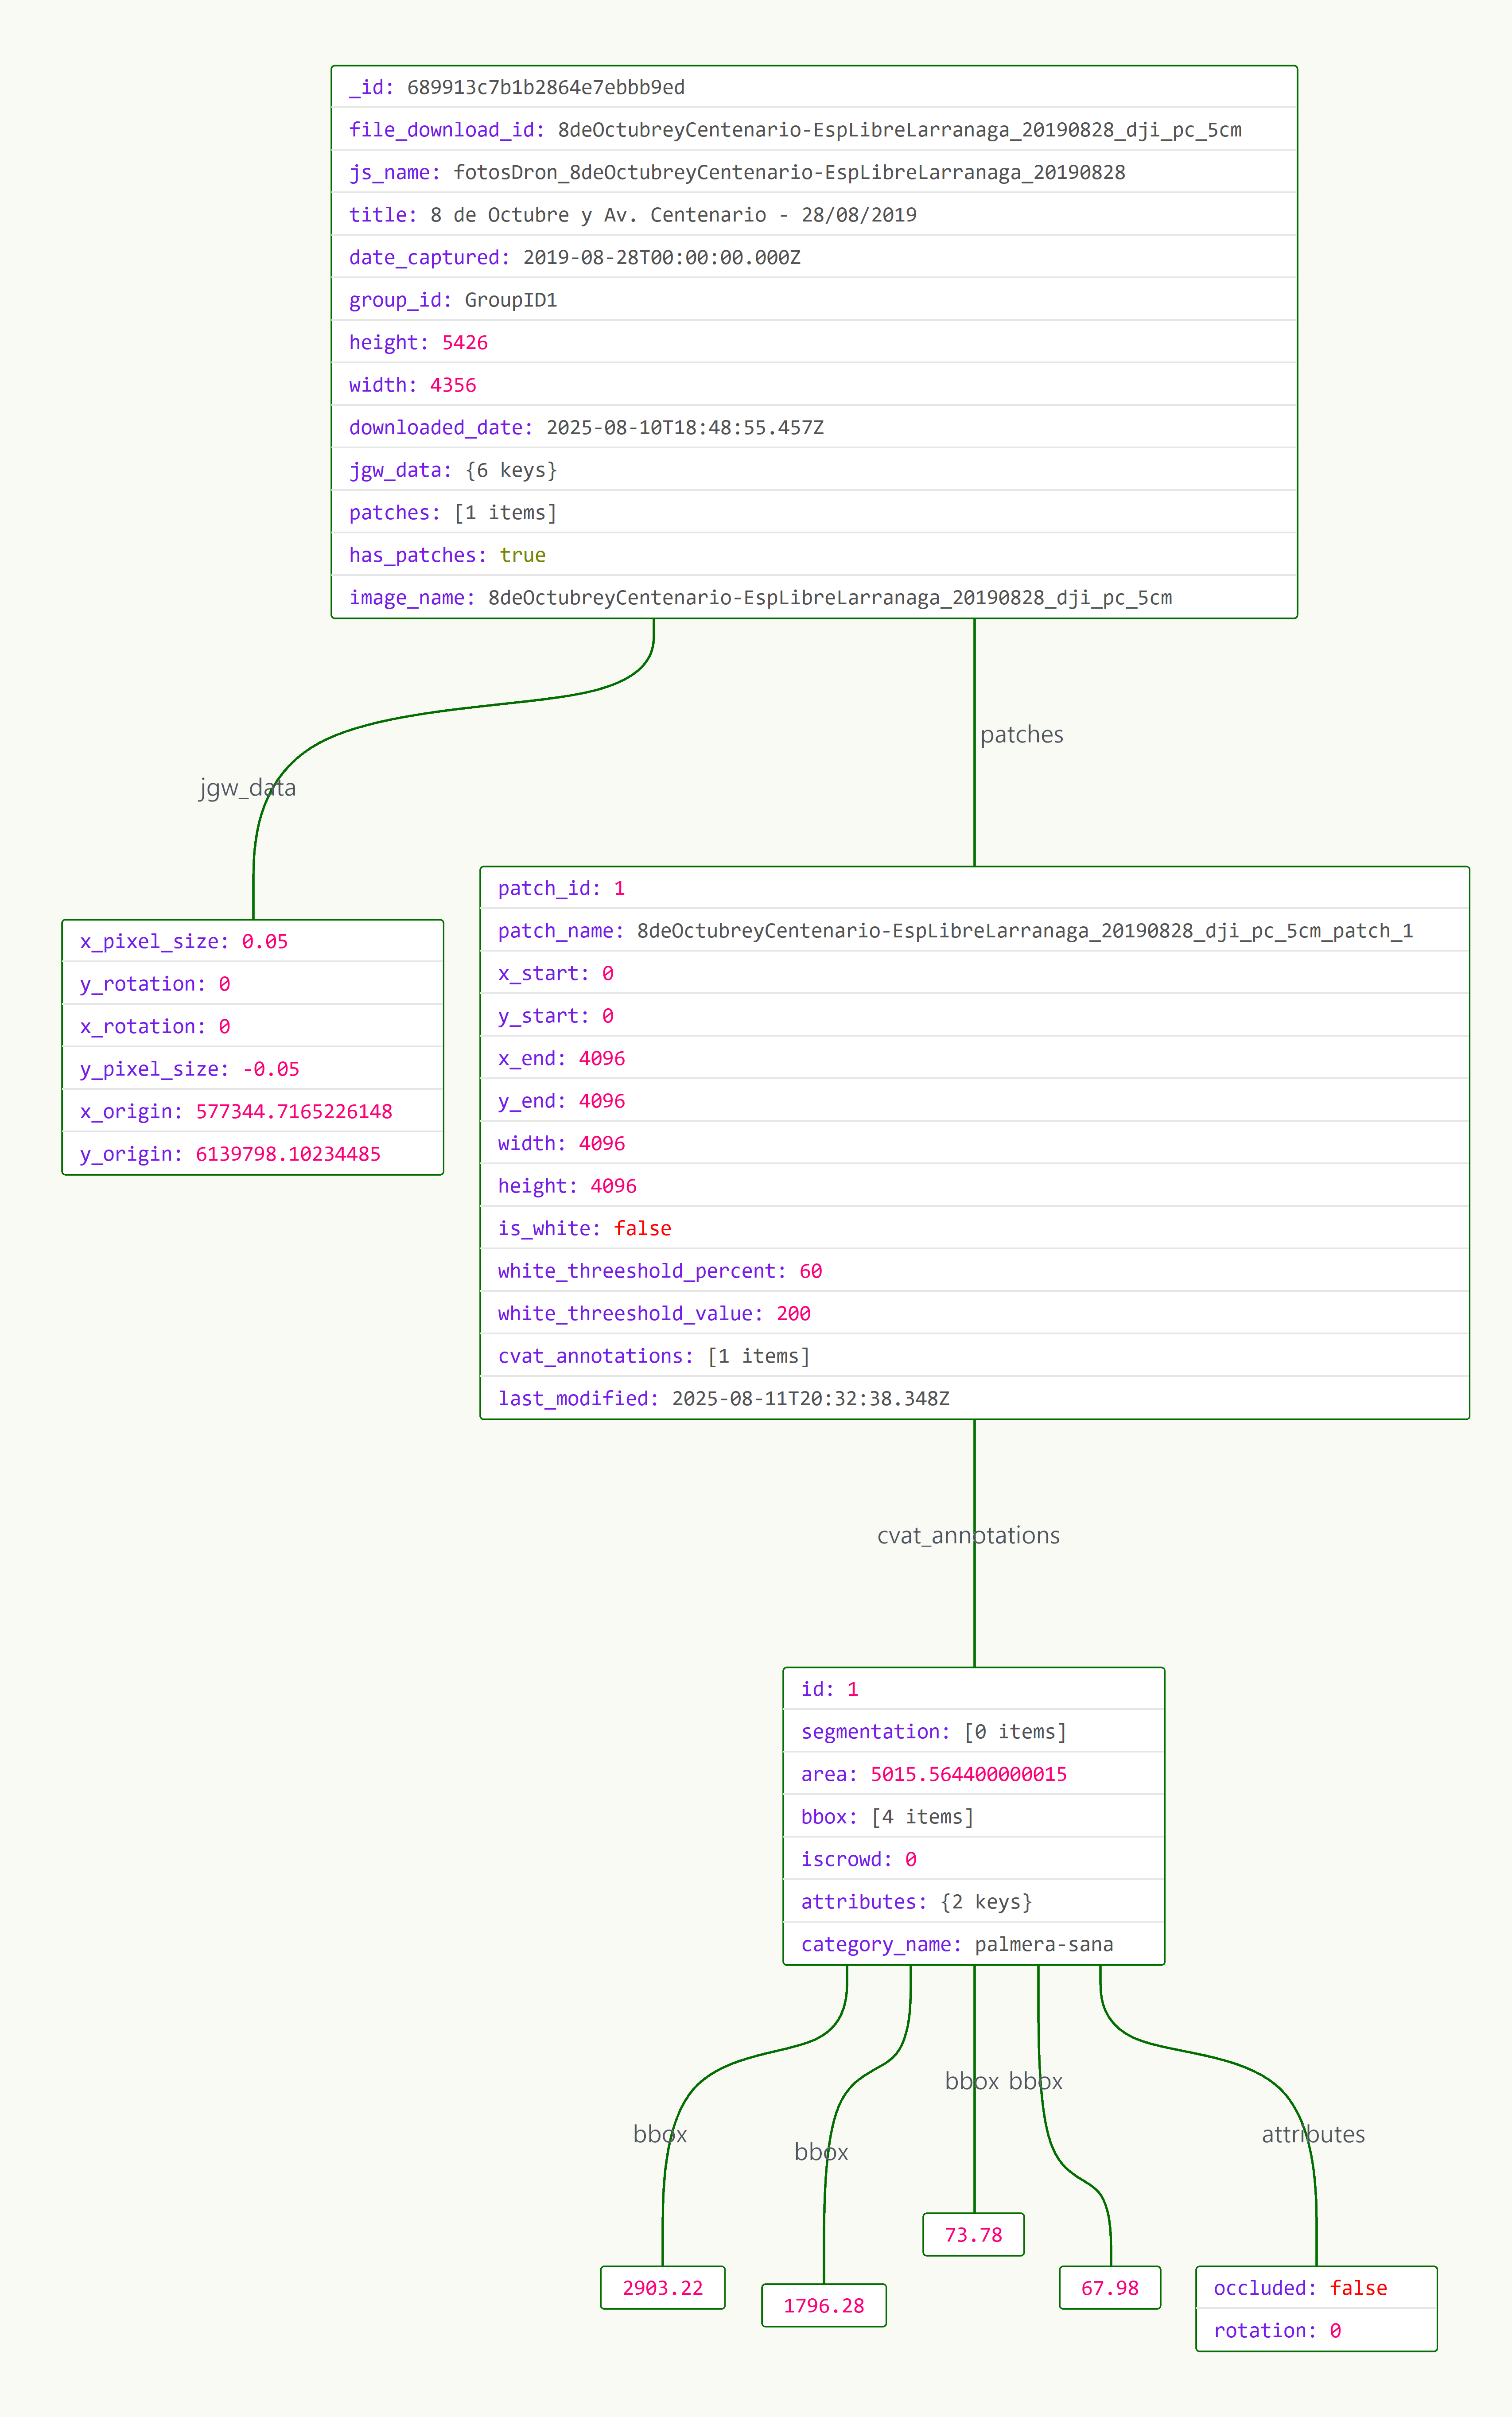
\includegraphics[scale=0.1]{./Figures/metadatos-mongodb.png}
  \caption{Estructura de los metadatos en MongoDB.}
  \label{fig:metadatos-mongodb}
\end{figure}

Un aspecto importante a destacar es el nodo \lstinline[language=sh]|jgw_data|. Este nodo contiene la información necesaria para georreferenciar la imagen, lo que permite que se pueda ubicar en un sistema de coordenadas geográficas. Esta información está adjunta con la imagen cuando se descarga desde el SIG.

Una vez que se completó la descarga de las imágenes, se procedió a la carga de las mismas en CVAT para su posterior etiquetado. Este proceso se realizó de manera manual, utilizando la interfaz gráfica de CVAT para seleccionar y cargar las imágenes desde MinIO. Se creó un proyecto en CVAT llamado "picudo-rojo-3cm-5cm" y se agregaron las imágenes correspondientes a este proyecto. Este proceso fue sencillo y eficiente, gracias a la integración entre CVAT y MinIO, que permitió una gestión fluida de las imágenes.

%----------------------------------------------------------------------------------------
%	SECTION 4
%----------------------------------------------------------------------------------------

\section{Proceso de etiquetado de datos}
\label{sec:etiquetado}

% Hablar de los tipos de usuarios, las pruebas que se realizaron -de control, no en profundidad- y las jornadas de etiquetado.
% También como se midió el progreso. Hablar del enfoque que se tomó (recortar las imágenes).
% Mostrar algunos de los etiquetados finales.
% Hablar de porque no se utlizó la información georreferenciada de las palmeras (los recortes no eran exactos).
% Hablar de algunas funciones de CVAT.
% Comunicaciones.

El proceso de etiquetado de datos fue una etapa crucial. Inicialmente, se intentó utilizar la información georreferenciada de las palmeras proporcionada por la IM. Sin embargo, se descubrió que los recortes de las imágenes no eran exactos, lo que dificultaba la identificación precisa de las palmeras en las imágenes ortorectificadas, debido a la gran variedad de tamaños, formas y colores que presentan las palmeras en las imágenes aéreas. La principal tarea en este caso era la de ajustar y verificar las coordenadas de las palmeras en las imágenes, lo que resultó ser un proceso laborioso y propenso a errores. Por lo tanto, se decidió optar por un enfoque manual para el etiquetado de las imágenes.Para esto, se contaba con el apoyo de un equipo de ingenieros agrónomos del sector de arbolado de la IM. Específicamente, se contó con la colaboración de cuatro ingenieros agrónomos, quienes tenían experiencia en el manejo y cuidado de palmeras, lo que resultó fundamental para la correcta identificación y etiquetado de las mismas en las imágenes ortorectificadas.

Se definieron los usuarios y roles, se cargaron los \textit{tasks} de CVAT y se dejó en libertad que cada usuario trabajara a su ritmo, asignándose un \textit{job} según sus necesidades. Se realizaron varias jornadas de etiquetado, en donde se evacuaron dudas y se definieron lineamientos para el etiquetado. Se establecieron cuatro clases de etiquetas: "palmera-sana", "palmera-infectada", "palmera-muerta" y "palmera exterminada". Un ejemplo de cada clase puede observarse en la figura \ref{fig:clases-palmeras}.

% TODO: Crear figura de las clases de palmeras
\begin{figure}[H]
  \centering
  
\includegraphics[scale=0.5]{./Figures/place-holder.png}
  \caption{Ejemplos de las clases definidas para el etiquetado de palmeras.}
  \label{fig:clases-palmeras}
\end{figure}

CVAT tiene la ventaja de permitir definir atributos para cada etiqueta. Utilizando esta funcionalidad, se definieron los atributos \lstinline[language=sh]|especie| y \lstinline[language=sh]|borroso|. El primero se definió como una lista de todas las especies de palmeras identificadas en Montevideo, el segundo siemplemente para marcar si la palmera estaba borrosa o no, en casos donde hubiese alguna duda.

La comunicación fue un aspecto fundamental durante el proceso de etiquetado. Se utilizó una combinación de correos electrónicos, manuales, reuniones presenciales y un grupo de \textit{whatsapp} para mantener una comunicación fluida entre los miembros del equipo. Esto permitió generar un consenso sobre las mejores prácticas para el etiquetado y resolver dudas de manera rápida y eficiente, aumentando la calidad de los datos etiquetados.

Aún con todo el apoyo brindado, la tarea de etiquetado resultó ser más desafiante de lo esperado. La complejidad de las imágenes, la variabilidad en la apariencia de las palmeras y la necesidad de un etiquetado preciso hicieron que el proceso fuera laborioso y requiriera una atención meticulosa a los detalles. Esto llevó a que el progreso del etiquetado fuera más lento de lo anticipado, lo que impactó en los plazos del proyecto. A pesar de estos desafíos, se logró avanzar significativamente en el etiquetado de las imágenes, lo que sentó las bases para el desarrollo de los modelos de detección.

Se etiquetaron un total de 1.663 imágenes, en donde se identificaron cerca de 6.000 palmeras. Un resumen detallado se puede observar en la tabla \ref{tab:resumen-imagenes-etiquetado}.

% TODO: Crear tabla resumen del etiquetado

La cantidad de etiquetas de la clase "palmera-sana" con respecto a las demás, se debe a que la mayoría de las imágenes fueron tomadas antes de la llegada del picudo rojo. En este punto se identificó un grave problema, en donde no se iba a lograr obtener una cantidad suficiente de detecciones con palmeras infectadas, muertas o exterminadas, lo que implicó utilizar otros enfoques para el entrenamiento de los modelo que se explican en siguiente capítulo.

Es muy difícil obtener una métrica certera de cuantas etiquetas por imagen se realizaron, dado que no todas las imágenes tienen palmeras y algunas tienen muchas más que otras. Sin embargo, se pudo evidenciar que hay imágenes que llegaban a contener hasta 50 palmeras, lo que da una idea de la complejidad del trabajo realizado. Estos datos se pudieron obtener utilizando la herramienta FiftyOne, que permite analizar y visualizar los datos de manera sencilla. Un resumen del proceso de etiquetado se puede observar en la tabla \ref{tab:resumen-etiquetado}

% TODO: Crear tabla de tiempos de etiquetado

Un ejemplo de una imagen etiquetada en CVAT se puede observar en la figura \ref{fig:imagen-etiquetada-cvat}.

% TODO: Crear figura de una imagen etiquetada en CVAT
\begin{figure}[H]
  \centering
  
\includegraphics[scale=0.2]{./Figures/place-holder.png}
  \caption{Ejemplo de una imagen etiquetada en CVAT.}
  \label{fig:imagen-etiquetada-cvat}
\end{figure}

%----------------------------------------------------------------------------------------
%	SECTION 5
%----------------------------------------------------------------------------------------

\section{Desarrollo de la aplicación web}
\label{sec:app_web}

En paralelo al proceso de etiquetado, se desarrolló la aplicación web principal del sistema, llamada "Mis palmeras". Esta aplicación tiene como objetivo principal mostrar los resultados de la detección del picudo rojo en las palmeras, utilizando las imágenes aéreas y los modelos de detección desarrollados. El prinicpal caso de uso en donde interactúa la plataforma se puede observar en la figura \ref{fig:caso-uso}.

% TODO: Crear figura del caso de uso principal de la plataforma
\begin{figure}[H]
  \centering
  
\includegraphics[scale=0.12]{./Figures/place-holder.png}
  \caption{Diagrama del caso de uso principal de la plataforma.}
  \label{fig:caso-uso}
\end{figure}

En esta linea, el valor final al usuario es un mapa con las palmeras detectadas, clasificadas por su estado de salud. Esta información se puede descargar en un KML para importar en otras herramientas utilizadas por varios equipos que gestionan la expansión de la plaga. También se puede descargar la imagen para verificar la visualización de las detecciones.

El desarrollo de la aplicación web se realizó utilizando Angular para el frontend y FastAPI para el backend. Se utilizó Keycloak como capa de autenticación y autorización, lo que permite gestionar los usuarios y sus permisos de manera segura. La aplicación web se diseñó para ser intuitiva y fácil de usar, con una interfaz gráfica que permite a los usuarios navegar por el mapa, visualizar las palmeras detectadas y acceder a la información detallada sobre cada una de ellas. El diagrama de flujo de la figura \ref{fig:diagrama-flujo-app} muestra el flujo de datos entre el backend y frontend. Actualmente la aplicación no cuenta con una base de datos, dado que las predicciones son "on-the-fly", es decir, se realizan en el momento en que el usuario solicita la información. Esto permite reducir la complejidad del sistema y evitar la necesidad de mantener una base de datos adicional. Sin embargo, en futuras versiones se podría considerar la incorporación de una base de datos para almacenar las predicciones y mejorar el rendimiento del sistema, que actualmente se manejan en memoria del backend.

% TODO: Crear figura del diagrama de flujo de la aplicación web
\begin{figure}[H]
  \centering
  
\includegraphics[scale=0.12]{./Figures/place-holder.png}
  \caption{Diagrama de flujo de la aplicación web.}
  \label{fig:diagrama-flujo-app}
\end{figure}

Un desafío importante en el desarrollo de la aplicación web fue la integración con los modelos de detección del picudo rojo. Actualmente la integración está áltamente acoplada 

Finalmente, en la figura \ref{fig:app-web} se puede observar una captura de pantalla de la aplicación web "Mis palmeras", mostrando el mapa con las palmeras detectadas y su estado de salud para un caso específico.

\begin{figure}[H]
  \centering
  
\includegraphics[scale=0.2]{./Figures/place-holder.png}
  \caption{Captura de pantalla de la aplicación web "Mis palmeras".}
  \label{fig:app-web}
\end{figure}
